\section{Theory}
%\label{sec:problem_description}
In Experiment A1, the basic equations are Bernoulli's \eqref{Bernoulli} .
%and the continuity equation.
\begin{equation}
\label{Bernoulli}
\left[ \frac{p}{\gamma}+\frac{v^2}{2g}+z \right]_1 = 
\left[ \frac{p}{\gamma}+\frac{v^2}{2g}+z \right]_2 
\end{equation}
As shown in the figure below, where 1 and 2 represent the surface of 
the reservoir and the water discharge point.
\begin{figure}[htb] % Here, top, bottom priority list
    \centering
    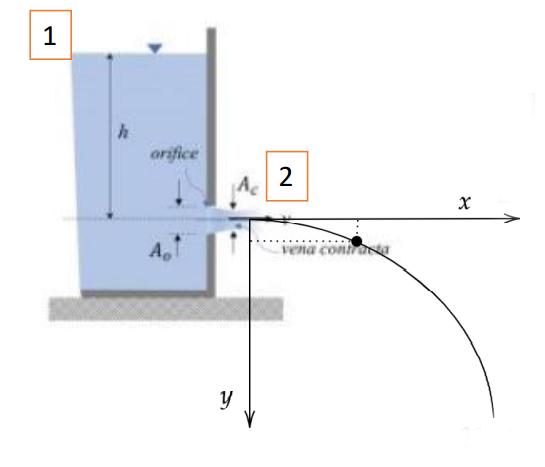
\includegraphics[scale=0.45]{Theory/figures/figure1.png}
    \caption{Experimental Demonstration}
    \label{fig:demo}
\end{figure}
%In Bernoulli's equation, because the position 1 is in contact with the air and the water surface is static, 
%so the pressure force p = 0, and the water surface flow velocity v = 0. 
%Similarly, the pressure at position 2 is p = 0. 
%With the datum at 2, we only need to measure the head difference between position 1 and 2, 
%and measure the jet velocity of 2, after that put into other constants, 
%Bernoulli's equation could be proved.
Because $p_1=0$ $p_2=0$ $v_1=0$ $z_1-z_2=h$, Bernoulli's equation can be simplified as
\begin{equation}
v_2=\sqrt{2gh}
\label{1}
\end{equation}
Where $v_2$ is the water velocity in position 2, h is the head difference between 1 and 2.
In fact, due to the jet vena contracta, it exists a coefficient $C_v$ to effect the real velocity.
$C_v$ depends on the viscosity of the water, so $C_v < 1$.
\begin{equation}
    v=C_v\sqrt{2gh}
    \label{2}
\end{equation}
By neglecting the air resistance, the x and y position could be caculated By

$ x=vt$ $y=\frac{1}{2}gt^2$

Hence,
\begin{equation}
    C_v=\frac{x}{2\sqrt{yh}}
    \label{5}
\end{equation}
Also can be rewrite as
\begin{equation}
    x=2C_v\sqrt{yh}
    \label{6}
\end{equation}
Hence, For a constant coefficient $C_v$, which can be determined from the x and y coordinates.
In Experiment A2, the continuity equation is given by
\begin{equation}
\label{velocity}
Q=Av
\end{equation}
%From this, we can calculate the real water flowrate.
%Because the vena contracta decrease the cross-sectional area of jet flow,
It also exists a coefficient $C_c$, which $C_c < 1$. Hence,
\begin{equation}
    \label{11}
    A=C_cA_0
\end{equation}
Substitution for v from \eqref{2}, the results is
\begin{equation}
    \label{13}
    Q_t=C_cA_0C_v\sqrt{2gh}=C_dA_0\sqrt{2gh}
\end{equation}
Which used the discharge coefficient$C_d$ to Substitute $C_c$ and $C_v$.($C_d=C_c*C_v$)
This is also a linear equation with horizontal 
coordinates $\sqrt{h}$ and vertical coordinates $Q_t$. The slope S =
$C_dA_0\sqrt{2g}$.

%Notice:  the water jet velocity measured by experiment A exists a 
%certain error.
%The flow rate measured by experiment A2 is a relatively smaller error.
%(see in section: Analysis %\autoref{sec:analysis}
%)

